\documentclass{article}

\author{Author: Jeremy Greenburg \\ Mentor: Dr. Joshua Guerin \\ Second Reader: Bob Bradley}
\title{The God Core \\ A Science Fiction Video Game Developed in C++}

% For importint code and text files
\usepackage{listings}
% For enumerating the Table of Contents
\usepackage{enumitem}
% Incase I need pictures
\usepackage{graphicx}

%Mathematics Galore
\usepackage{amsmath}
\usepackage{amsfonts}
\usepackage{amssymb}
\usepackage{gensymb}

\usepackage{fullpage}

\usepackage{csvsimple}
\usepackage{longtable}

% Subsection numbering
\setcounter{secnumdepth}{3}

% Only Subsections in Table of Contents
\setcounter{tocdepth}{2}

\begin{document}
\maketitle
\pagebreak

\tableofcontents

\pagebreak

\section{Preamble}

\section{Programming}

\subsection{The Language}

\subsection{APIs}

\subsubsection{OpenGL}
OpenGL, or the Open Graphics Library, is one of the most popular graphics libraries out there. It gives access to linear algebra functions for matrix manipulation (which is important, as 3D graphics relies heavily upon matrix transformations), keyboard and mouse input, and windowing. I chose to use OpenGL over a different graphics library, such as Microsoft's DirectX, because it is open source and cross platform, which would make porting my game to a different Operating System a much easier task if I ever decide to in the future.

\subsubsection{SOIL}
SOIL, or the Simple OpenGL Interface Library, is a small extension to OpenGL that I picked up along the way. It is a texture library that can load .jpg and .png images and bind them to an OpenGL texture, making it very simple to incorporate such images into my game.

\subsubsection{FMOD}
I chose FMOD as the base for my game's audio as it is a simple, lightweight, and free to use sound API, and most other audio APIs that I looked at lacked support for MP3 files. 

\subsubsection{SQlite}
I decided to use SQLite for my database because it is a lightweight simplified version of a SQL database, allowing the game data to be stored and embedded in the application without taking much room or take a great deal of time to perform a query.

\subsection{Game Engine}

I crafted the engine of my game in C++ over two years starting in my second semester sophomore year and ending the first semester of my senior year. It consists of 53 C++ files and was developed in Microsoft Visual Studio. The code can be found in the Appendix of this writeup or it can be located on GitHub at \emph{https://github.com/Jerrgree/The-God-Core-Source}. The game can also be installed at GitHub.

\subsubsection{Rectangles and Triangles}
Rectangles and triangles are the two fundamental polygons that build up my game. Rectangles in particular make up the walls, floors, ceilings, doors, terminals, and most of the HUD and menu. They started as simply two arrays- one that holds all 9 (for triangles) or 12 (for rectangles) values describing the coordinates in the game that they inhabit, as well as a 4 value vector containing the objects RGBA values.

For collision purposes, when a rectangle class is expanded with the ability to calculate and store its norm and Plane equation (Form $ax + by + cz + d = 0$).

This equation is calculated using the any three corners of the rectangle (Calling them A, B, and C) as follows:

\noindent
$
\vec{AB} = \left| \begin{array}{c}
Bx - Ax \\
By - Ay \\
Bz - Az
\end{array} \right|
\vec{AC} = \left| \begin{array}{c}
Cx - Ax \\
Cy - Ay \\
Cz - Az
\end{array} \right| \\
a = \vec{AB}_2 * \vec{AC}_3 - \vec{AB}_3 * \vec{AC}_2 \\
b = \vec{AB}_3 * \vec{AC}_1 - \vec{AB}_1 * \vec{AC}_3 \\
c = \vec{AB}_1 * \vec{AC}_2 - \vec{AB}_2 * \vec{AC}_1 \\
d = aAx + bAy + cAz
$

\emph{\tiny{Formula obtained from http://keisan.casio.com/exec/system/1223596129}}

The norm of the plane can then be derived using the equation $\sqrt{a^2 + b^2 + c^2}$

\subsubsection{In Game Terminals}
In game terminals are each bound to a \emph{terminal file}, a unique file that contains the contents of its respective terminal.

The terminal file is divided into two sections: the file names and the file contents. This is an example terminal file:

\lstinputlisting[
basicstyle=\ttfamily \small,
numbers=left,
breaklines=true,
linerange={1-1000},
firstnumber = 1]{../Resources/Text/test.tm}

The program parses the file by first separating the in game content (the bracketed number and name) that should be displayed to the user from it's tag. The tags are stored in an array, where its index is equal to the bracketed number. The help display is always stored at the 0th index.

Then, whenever the player types in a read command (E.G. Read 1), the program will send the terminal file and the correct tag to the text engine for the content to be displayed to the screen.

\subsubsection{Triggers and Switches}
Triggers are a more sophisticated way to implement interaction between two different objects. The implementation was designed to be abstracted away from object types so that, in theory, any arbitrary object could activate another, but in practice due to the few classes of objects in my game, it served as a way for terminals to power switches on. 

The trigger class works by holding two void pointers, one for a triggering object and one for the target object. It also holds the object types (defined in GCTypes.h) of each object. Whenever an object is interacted with, every trigger in the game is attempted to be triggered \textbf{(trying to find better phrasing here)} and if the object is the same as the trigger pointer (no referencing needed as the pointers will always be equal), the target is dereferenced according to the appropriate type and activated.

It holds very similar function to a switch, the primary difference being that the switch is a tangible object in the game with the triggering object being itself, and the triggers being an intangible association between two objects. If I had more time in development, I would have liked to refactor much of the switch's internal functionality so that it is simply an object, with the actual interaction between the switch and it's target taking place as a trigger, but the conception and implementation of triggers came too late in development and implementing the switch change would require a good deal of code and data rewrites.

\subsubsection{Camera Control}
The CameraControl class is designed to control and manipulate the player's perspective as they navigate through the game. It contains two ordered triples of floating point numbers: The xyz location of the player, and the rotation along the x axis (looking left/right), the y axis (up/down), and the z axis (barrel roll). It also contains two additional floating point values, the movement speed and the turning speed. 

The player can move forwards and backwards, as well as strafe left and right. To correctly formulate the player's movement, I had to envision a circle centered on the player with a radius of the player's movement speed. Based on the angle from the x and z rotation, the next place that the player move is simply a spot on the circumference of the circle based on the rotation angle, and moving forward can be derived from this formula:

z := z $\pm$ moveSpeed * cos(radian(x\_angle))

x := x $\mp$ moveSpeed * sin(radian(x\_angle))

\emph{\tiny{Formula obtained from Robert De Yoso}}

\small{}

Following that formula, it's simple to implement movement to the left, right by adding or subtracting 90$\degree$, and backwards movement by adding 180$\degree$.

Whenever OpenGL renders a new frame, the 'camera' is always returned to the origin of the map, so after drawing the level and before flushing the buffer, the Camera Control calls glTranslate to move the camera to the correct location, and then calls glRotate 3 times, once for each axis, to orient the camera in the correct direction.

\subsubsection{Heads Up Display}
The Heads Up Display is drawn after the level is draw, so that it overlays information to the player. It primarily is used to add a bit of flavor to the game by drawing the helmet for the player, but it also serves to display the developer console when activated.

The display also delivers a prompt to the user whenever they are in range of an object that can be interacted with.

\subsubsection{2D}
As multiple different objects required the ability to \textbf{2D IT UP CHANGE THIS SOON}, I extracted the ability to draw in 2D into it's own class and it was inherited whenever it was needed.

To convert OpenGL into 2D frame, I needed to first disable lighting, depth testing and depth masking. Next I pushed an \emph{orthogonal} matrix onto OpenGL's matrix stack using the length and width of the screen so that all matrix transformations corresponded to a pixel on the screen. Re-enabeling 3D is as simple as popping the orthogonal matrix from the stack and re-enabling depth testing and masking.

\subsubsection{Collision Engine}
This determines when the player has collided with an object in the world. There are two types of collisions: player-object collisions and player-wall collisions.

Player object collisions are simple to detect, as both the player and the object can be placed within imaginary "bounding spheres" that extend around the player and object. Collision can be detected with this formula:
$\sqrt{(x_2 - x_1) + (y_2 - y_1) + (z_2 - z_1)} < r_2 + r_1$
If the distance between the two spheres is less than the sum of the radii of the two spheres, the they must be colliding.

Player-wall collisions were much harder to reconcile. Because walls tend to be long and thin, you can't simply place one within a bounding sphere, the resulting sphere would simply be too massive.

To rectify that, the collision is split into two phases: broad and narrow.

In the broad phase, we use the plane equation $ax + by + cz + d$ that is derived in the Rectangle section. We use the formula $\frac{ax + by + cz + d}{\sqrt{a^2 + b^2 + c^2}}$, where x, y, and z are the player's x, y, and z coordinates. If the resulting value is less than the radius of the player's bounding sphere, the player has hit that plane and we move onto the narrow phase.

In the narrow phase, each wall is aligned on an axis: x, y, or z. We simply take the largest and smallest values of the coordinates on that axis (for instance, if the wall is x aligned, we take the largest and smallest x value). If the sphere is in between the two values, the player has hit the wall. Otherwise, they hit the plane but not the wall.

\subsubsection{MusicManager}
To play background music, I used the FMOD low level API for C++. FMOD can dynamically load and play as multiple sounds, which can either be set to loop (such as background music) or not to loop (for sound effects). Proper memory management is important, as the individual sounds are dynamically created outside of the Music Manager class and must be allocated and deallocated properly to avoid memory leaks.

\subsubsection{TextEngine}
The Text Engine was constructed to handle displaying all text to the screen. It uses OpenGL's glutBitmapCharacter function to display clear, concise text.

Every function to display text takes two coordinates (the x,y coordinates on the screen to start displaying the text), and the RGB color values for the text. There are two functions for displaying text, the simpler one merely takes in a string and prints it on the corresponding location on the screen. The more complex function takes in a file and a content tag. The files are structured like so:

\lstinputlisting[
	basicstyle=\ttfamily \small,
	numbers=left,
	breaklines=true,
	linerange={1-1000},
	firstnumber = 1]{../Resources/Text/test.txt}
	
The Text Engine searches through the designated file line by line until it discovers the line containing the proper tag. Then, until it reaches the closing 'END' tag, it stores every line inside of a vector. Once it has retrieved all of the necessary content, it starts to display the text to the screen line by line, starting from the designated XY position and increasing the Y value for each line.

\subsubsection{Game Saving and Loading}

\subsubsection{Keyboard}
The Keyboard class primarily serves to encapsulate the OpenGL callbacks that receive keystrokes: the normal function that accepts all alphanumeric and punctuation, and the special function that handles function keys and escape. However, there is a minor bit of overhead that goes into deciding where the input goes.

Under normal circumstances, the only normal keystrokes accepted are the WASD keys for movement, the E key for interaction, and the '~' key for toggling the development console.

When in either a terminal or the development console, all keys are immediately concatenated to an input string with the exception of the '~' which will close the development console, or the enter key which will send the input string to it's appropriate destination to be parsed and interpreted, after which the input string is cleared so that a new command can be entered.

Also accepted are the up and down arrow keys, which will cycle through the console/terminals command history.

\subsubsection{Level Loading and displaying}
Loading each level involves a series of SQL queries through the SQLite API. Loading each level first involves opening a connection with the database, and retrieving all data from each table in the database in turn. All important data from the database is stored in a class of the appropriate type, unnecessary data is discarded, and in the end each class is pushed into a vector of the appropriate type. 

The data is loaded in a strict order, due to some objects having dependencies on others (that is, some objects require other objects to already exist). Thus the first things that are loaded are purely independent objects, all doors, walls, and terminals. Next switches are loaded, because they require both doors and terminals to already exist. Finally, the triggers are loaded, because they require both switches and terminals.

When loading switches and triggers, the objects also need to be \emph{bound} to their appropriate target. This is why doors, switches, and terminals all carry their ID's into the program with them, while triggers and walls discard their ID. Once all of the objects that need to be bound are loaded into the game, the game proceeds to bind them to their target. For each switch that needs to be bound, the game loops through either the list of terminals or the list of doors for the appropriate object and creates a pointer to that object inside of the switch, thus ensuring that the switch can toggle its target instantly without needing to search every time it is triggered. The triggers are bound similar, with the difference that each object must perform two searches, one for the triggering object and one for the target object.

If there is any data error in regards to binding --- that is, and object attempts to bind to an object that does not exist, the error is considered fatal and the game immediately shuts down after logging the error.

The OpenGL display function calls upon the Level class to display all in game objects. This is a simple matter, because each object has it's own function to display itself. Thus it is a simple matter to loop through each vector and tell each object to display itself.

\subsubsection{Console and Logging}

\section{Appendices}

\subsection{Source Code}

\subsubsection{main.cpp}
	\lstinputlisting[
				basicstyle=\ttfamily \small,
				numbers=left,
				breaklines=true,
 				linerange={1-1000},
 				firstnumber = 1]{../main.cpp}
 				
\subsubsection{CameraControl.h}
	\lstinputlisting[
					basicstyle=\ttfamily \small,
					numbers=left,
					breaklines=true,
					linerange={1-1000},
					firstnumber = 1]{../CameraControl.h}

\subsubsection{CameraControl.cpp}
	\lstinputlisting[
					basicstyle=\ttfamily \small,
					numbers=left,
					breaklines=true,
					linerange={1-1000},
					firstnumber = 1]{../CameraControl.cpp}
					
\subsubsection{CollisionEngine.h}
	\lstinputlisting[
					basicstyle=\ttfamily \small,
					numbers=left,
					breaklines=true,
					linerange={1-1000},
					firstnumber = 1]{../CollisionEngine.h}
					
\subsubsection{CollisionEngine.cpp}
	\lstinputlisting[
					basicstyle=\ttfamily \small,
					numbers=left,
					breaklines=true,
					linerange={1-1000},
					firstnumber = 1]{../CollisionEngine.cpp}
					
\subsubsection{Console.h}
	\lstinputlisting[
					basicstyle=\ttfamily \small,
					numbers=left,
					breaklines=true,
					linerange={1-1000},
					firstnumber = 1]{../Console.h}
					
\subsubsection{Console.cpp}
	\lstinputlisting[
					basicstyle=\ttfamily \small,
					numbers=left,
					breaklines=true,
					linerange={1-1000},
					firstnumber = 1]{../Console.cpp}
					
\subsubsection{Cylinder.h}
	\lstinputlisting[
					basicstyle=\ttfamily \small,
					numbers=left,
					breaklines=true,
					linerange={1-1000},
					firstnumber = 1]{../Cylinder.h}
					
\subsubsection{Cylinder.cpp}
	\lstinputlisting[
					basicstyle=\ttfamily \small,
					numbers=left,
					breaklines=true,
					linerange={1-1000},
					firstnumber = 1]{../Cylinder.cpp}
					
\subsubsection{Door.h}
	\lstinputlisting[
					basicstyle=\ttfamily \small,
					numbers=left,
					breaklines=true,
					linerange={1-1000},
					firstnumber = 1]{../Door.h}

\subsubsection{Door.cpp}
	\lstinputlisting[
					basicstyle=\ttfamily \small,
					numbers=left,
					breaklines=true,
					linerange={1-1000},
					firstnumber = 1]{../Door.cpp}
 				
\subsubsection{GameManager.h}
	\lstinputlisting[
					basicstyle=\ttfamily \small,
					numbers=left,
					breaklines=true,
	 				linerange={1-1000},
	 				firstnumber = 1]{../GameManager.h}

\subsubsection{GameManager.cpp}
	\lstinputlisting[
					basicstyle=\ttfamily \small,
					numbers=left,
					breaklines=true,
	 				linerange={1-1000},
	 				firstnumber = 1]{../GameManager.cpp}
	 				
\subsubsection{GCTypes.h}
	\lstinputlisting[
	 				basicstyle=\ttfamily \small,
	 				numbers=left,
	 				breaklines=true,
	 				linerange={1-1000},
	 				firstnumber = 1]{../GCTypes.h}
	 				
\subsubsection{Globals.h}
	 \lstinputlisting[
	 				basicstyle=\ttfamily \small,
	 				numbers=left,
	 				breaklines=true,
	 				linerange={1-1000},
	 				firstnumber = 1]{../Globals.h}
	 				
\subsubsection{Globals.cpp}
	 \lstinputlisting[
	 				basicstyle=\ttfamily \small,
	 				numbers=left,
	 				breaklines=true,
	 				linerange={1-1000},
	 				firstnumber = 1]{../Globals.cpp}
	 				
	 				
\subsubsection{HeadsUpDisplay.h}
	 \lstinputlisting[
					basicstyle=\ttfamily \small,
	 				numbers=left,
	 				breaklines=true,
	 				linerange={1-1000},
	 				firstnumber = 1]{../HeadsUpDisplay.h}
	 				
\subsubsection{HeadsUpDiplay.cpp}
	 \lstinputlisting[
					basicstyle=\ttfamily \small,
	 				numbers=left,
	 				breaklines=true,
	 				linerange={1-1000},
	 				firstnumber = 1]{../HeadsUpDisplay.cpp}		
	 				
\subsubsection{Keyboard.h}
	 \lstinputlisting[
					basicstyle=\ttfamily \small,
	 				numbers=left,
	 				breaklines=true,
	 				linerange={1-1000},
	 				firstnumber = 1]{../Keyboard.h}
	 				
\subsubsection{Keyboard.cpp}
	 \lstinputlisting[
					basicstyle=\ttfamily \small,
	 				numbers=left,
	 				breaklines=true,
	 				linerange={1-1000},
	 				firstnumber = 1]{../Keyboard.cpp}
	 				
\subsubsection{Level.h}
	 \lstinputlisting[
					basicstyle=\ttfamily \small,
	 				numbers=left,
	 				breaklines=true,
	 				linerange={1-1000},
	 				firstnumber = 1]{../Level.h}
	 				
\subsubsection{Level.cpp}
	 \lstinputlisting[
					basicstyle=\ttfamily \small,
	 				numbers=left,
	 				breaklines=true,
	 				linerange={1-1000},
	 				firstnumber = 1]{../Level.cpp}
	 				
\subsubsection{Logger.h}
	 \lstinputlisting[
	 				basicstyle=\ttfamily \small,
	 				numbers=left,
	 				breaklines=true,
	 				linerange={1-1000},
	 				firstnumber = 1]{../Logger.h}
	 				
\subsubsection{Logger.cpp}
	\lstinputlisting[
	 				basicstyle=\ttfamily \small,
	 				numbers=left,
	 				breaklines=true,
	 				linerange={1-1000},
	 				firstnumber = 1]{../Logger.cpp}
	 				
\subsubsection{MainMenu.h}
	\lstinputlisting[
					basicstyle=\ttfamily \small,
					numbers=left,
					breaklines=true,
					linerange={1-1000},
					firstnumber = 1]{../MainMenu.h}

\subsubsection{MainMenu.cpp}
	\lstinputlisting[
					basicstyle=\ttfamily \small,
					numbers=left,
					breaklines=true,
					linerange={1-1000},
					firstnumber = 1]{../MainMenu.cpp}	 
 				
\subsubsection{MusicManager.h}
	\lstinputlisting[
					basicstyle=\ttfamily \small,
					numbers=left,
					breaklines=true,
	 				linerange={1-1000},
	 				firstnumber = 1]{../MusicManager.h}
	 				
\subsubsection{MusicManager.cpp}
	\lstinputlisting[
					basicstyle=\ttfamily \small,
					numbers=left,
					breaklines=true,
	 				linerange={1-1000},
	 				firstnumber = 1]{../MusicManager.cpp}
	 				
\subsubsection{Plane.h}
	\lstinputlisting[
					basicstyle=\ttfamily \small,
	 				numbers=left,
	 				breaklines=true,
	 				linerange={1-1000},
	 				firstnumber = 1]{../Plane.h}
	 				
\subsubsection{Plane.cpp}
	\lstinputlisting[
					basicstyle=\ttfamily \small,
	 				numbers=left,
	 				breaklines=true,
	 				linerange={1-1000},
	 				firstnumber = 1]{../Plane.cpp}
	 			
\subsubsection{Return.h}
	\lstinputlisting[
	 				basicstyle=\ttfamily \small,
	 				numbers=left,
	 				breaklines=true,
	 				linerange={1-1000},
	 				firstnumber = 1]{../Return.h}
	 				
\subsubsection{Resource.h}
	\lstinputlisting[
					basicstyle=\ttfamily \small,
					numbers=left,
					breaklines=true,
					linerange={1-1000},
					firstnumber = 1]{../return.h}
	 				
\subsubsection{SaveManager.h}
	\lstinputlisting[
					basicstyle=\ttfamily \small,
					numbers=left,
					breaklines=true,
	 				linerange={1-1000},
	 				firstnumber = 1]{../SaveManager.h}
	 				
\subsubsection{SaveManager.cpp}
	\lstinputlisting[
					basicstyle=\ttfamily \small,
					numbers=left,
					breaklines=true,
	 				linerange={1-1000},
	 				firstnumber = 1]{../SaveManager.cpp}
	 				
\subsubsection{Switch.h}
	\lstinputlisting[
	 				basicstyle=\ttfamily \small,
	 				numbers=left,
	 				breaklines=true,
	 				linerange={1-1000},
	 				firstnumber = 1]{../Switch.h}
	 				
\subsubsection{Switch.cpp}
	\lstinputlisting[
	 				basicstyle=\ttfamily \small,
	 				numbers=left,
	 				breaklines=true,
	 				linerange={1-1000},
	 				firstnumber = 1]{../Switch.cpp}
	 				
\subsubsection{Terminal.h}
	\lstinputlisting[
					basicstyle=\ttfamily \small,
	 				numbers=left,
	 				breaklines=true,
	 				linerange={1-1000},
	 				firstnumber = 1]{../Terminal.h}
	 				
\subsubsection{Terminal.cpp}	
	\lstinputlisting[
					basicstyle=\ttfamily \small,
	 				numbers=left,
	 				breaklines=true,
	 				linerange={1-1000},
	 				firstnumber = 1]{../Terminal.cpp}
	 				
\subsubsection{TextEngine.h}
	\lstinputlisting[
					basicstyle=\ttfamily \small,
	 				numbers=left,
	 				breaklines=true,
	 				linerange={1-1000},
	 				firstnumber = 1]{../TextEngine.h}
	 				
\subsubsection{TextEngine.cpp}
	\lstinputlisting[
					basicstyle=\ttfamily \small,
	 				numbers=left,
	 				breaklines=true,
	 				linerange={1-1000},
	 				firstnumber = 1]{../TextEngine.cpp}
	 				
\subsubsection{Triangle.h}
	\lstinputlisting[
					basicstyle=\ttfamily \small,
	 				numbers=left,
	 				breaklines=true,
	 				linerange={1-1000},
	 				firstnumber = 1]{../Triangle.h}
	 				
\subsubsection{Triangle.cpp}
	\lstinputlisting[
					basicstyle=\ttfamily \small,
	 				numbers=left,
	 				breaklines=true,
	 				linerange={1-1000},
	 				firstnumber = 1]{../Triangle.cpp}
	 				
	 				
\subsubsection{Trigger.h}
	\lstinputlisting[
	 				basicstyle=\ttfamily \small,
	 				numbers=left,
	 				breaklines=true,
	 				linerange={1-1000},
	 				firstnumber = 1]{../Trigger.h}
	 				
\subsubsection{Trigger.cpp}
	\lstinputlisting[
	 				basicstyle=\ttfamily \small,
	 				numbers=left,
	 				breaklines=true,
	 				linerange={1-1000},
	 				firstnumber = 1]{../Trigger.cpp}
	 				
\subsubsection{Triple.h}
	\lstinputlisting[
	 				basicstyle=\ttfamily \small,
	 				numbers=left,
	 				breaklines=true,
	 				linerange={1-1000},
	 				firstnumber = 1]{../Triple.h}
	 				
\subsubsection{Triple.cpp}
	\lstinputlisting[
	 				basicstyle=\ttfamily \small,
	 				numbers=left,
	 				breaklines=true,
	 				linerange={1-1000},
	 				firstnumber = 1]{../Triple.cpp}
	 				
\subsubsection{TwoD.h}
	\lstinputlisting[
					basicstyle=\ttfamily \small,
					numbers=left,
					breaklines=true,
					linerange={1-1000},
					firstnumber = 1]{../TwoD.h}

\subsubsection{TwoD.cpp}	
	\lstinputlisting[
					basicstyle=\ttfamily \small,
					numbers=left,
					breaklines=true,
					linerange={1-1000},
					firstnumber = 1]{../TwoD.cpp}

\subsection{Database}
	
\subsubsection{Walls}

\tiny{}

\setlength{\tabcolsep}{2.5pt}
\csvautolongtable[respect all]{walls.csv}

\small{}
\subsubsection{Doors}
\csvautotabular[respect all]{doors.csv}

\subsubsection{Switches}
\csvautotabular[respect all]{switches.csv}

\subsubsection{Terminals}
\csvautotabular[respect all]{terminals.csv}

\subsubsection{Triggers}
\csvautotabular[respect all]{triggers.csv}

\tiny{}
\subsubsection{Cylinders}
\csvautotabular[respect all]{cylinders.csv}

\small{}
\subsection{Images}

\subsubsection{Main Menu}
	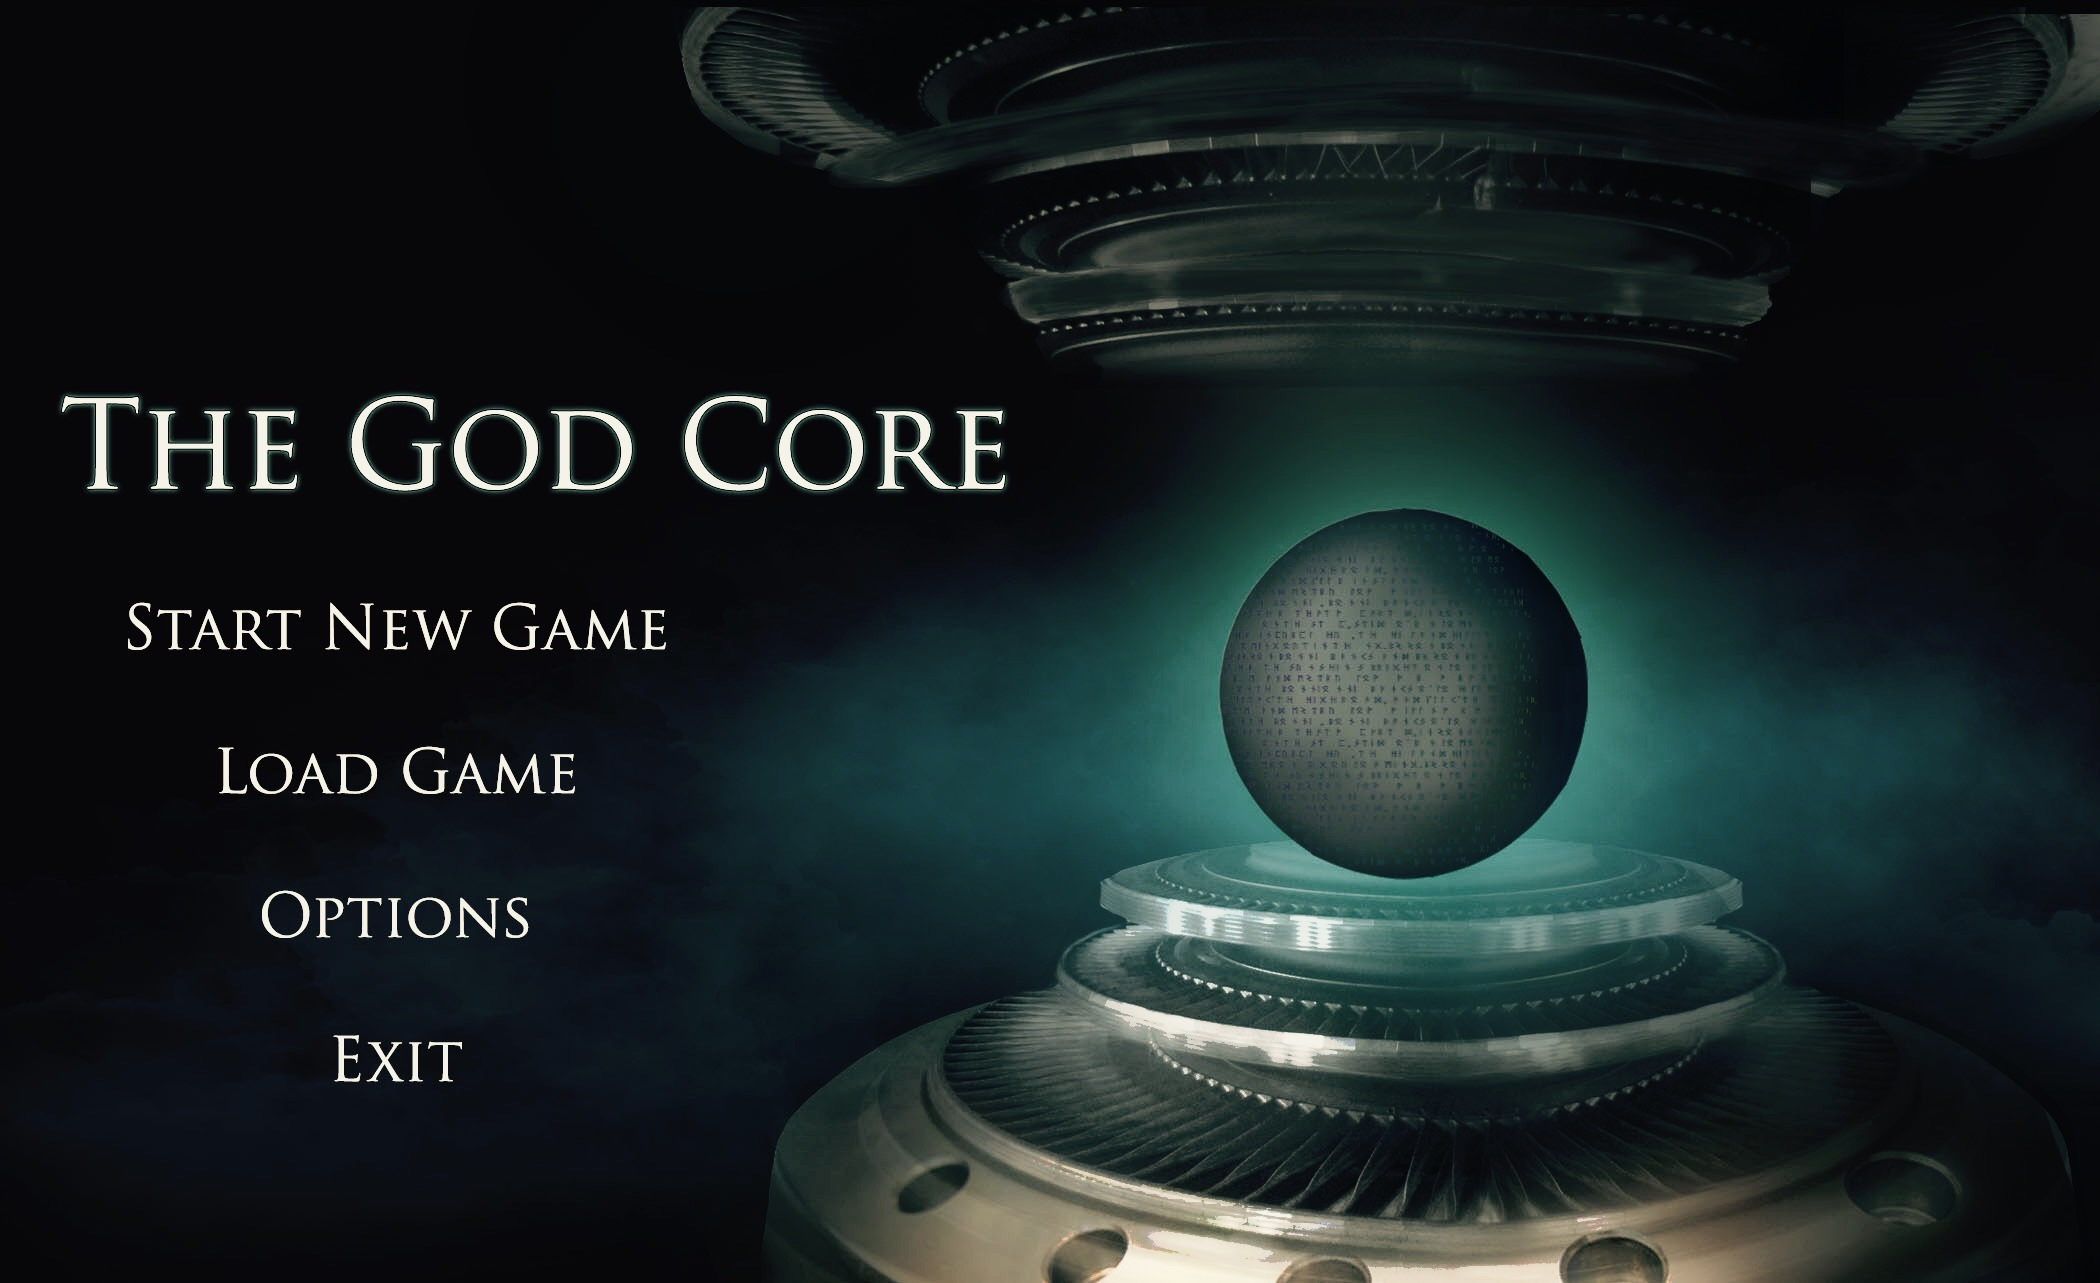
\includegraphics[width=18cm]{../Resources/Images/Main}
\subsubsection{Terminal Banner}
	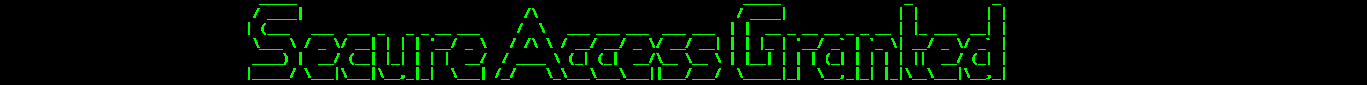
\includegraphics[width=18cm]{../Resources/Images/banner}
\subsubsection{Game Icon}
	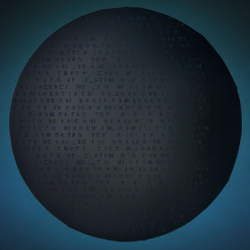
\includegraphics[width=5cm]{../Resources/Images/Core}
\subsection{Music}

\end{document}